%
% proposed-work.tex
%
% Copyright (C) 2021 by Universidade Federal de Santa Catarina.
%
% On-Board Data Processing Techniques to Improve the Performance of Small Satellites
%
% This work is licensed under the Creative Commons Attribution-ShareAlike 4.0
% International License. To view a copy of this license,
% visit http://creativecommons.org/licenses/by-sa/4.0/.
%

%
% \brief Proposed work section.
%
% \author Gabriel Mariano Marcelino <gabriel.mm8@gmail.com>
%
% \version 0.1.0
%
% \date 2021/06/14
%

\section{Proposed Work} \label{sec:proposed-work}

\begin{itemize}
    \item Explorar técnicas e métodos para aumentar a capacidade de proessamento embarcado em pequenos satélites
    \item Explorar técnicas de redução do consumo de energia durante o processamento, e consequentemente a eficiência energética do computador de bordo
    \item Para isso, levar em consideração as questões ambientais da operação de um satélite, como a incidência de radiação, que degrada o funcionamento de toda a eletrônica embarcada
\end{itemize}

\subsection{FloripaSat-2 Experiment}

Como um primeiro experimento para aplicar os conceitos aqui apresentados, pretende-se executar um experimento a ser embarcado no nanossatélite FloripaSat-2 \cite{floripasat2}.

The Radiation Monitor (or Harsh Payload) is a payload capable of evaluate the radiation effects on three SDRAM memories with different manufacturing nodes. This payload will test this chips in the real harsh space environment by flying aboard of FloripaSat-2 CubeSat mission. These particular SDRAM memories were previous characterized on laboratory experiments, then by exposing them to the real environments and executing the same tests routines will not only generate more results for analysis, but also provide an opportunity to assess the test methodologies themselves. Also, after collecting sufficient data to be analysed, this payload could be used to provide a meaningful health status, concerning the radiation doses which the satellite were exposed, to the entire satellite subsystems and further missions. A picture of the harsh payload board is available in \autoref{fig:harsh-payload-pcb}.

\begin{figure}[!ht]
    \begin{center}
        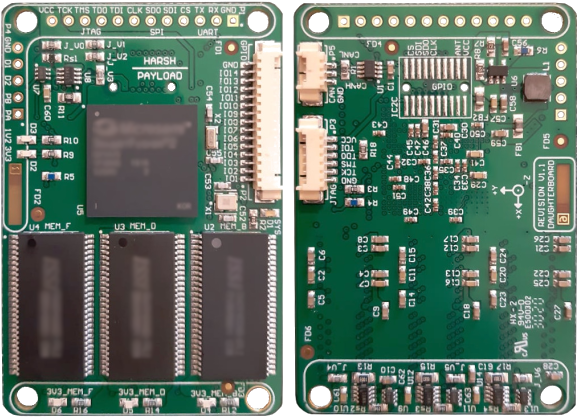
\includegraphics[width=0.8\columnwidth]{figures/harsh-payload}
        \caption{Harsh payload PCB.}
        \label{fig:harsh-payload-pcb}
    \end{center}
\end{figure}

\begin{figure}[!ht]
    \begin{center}
        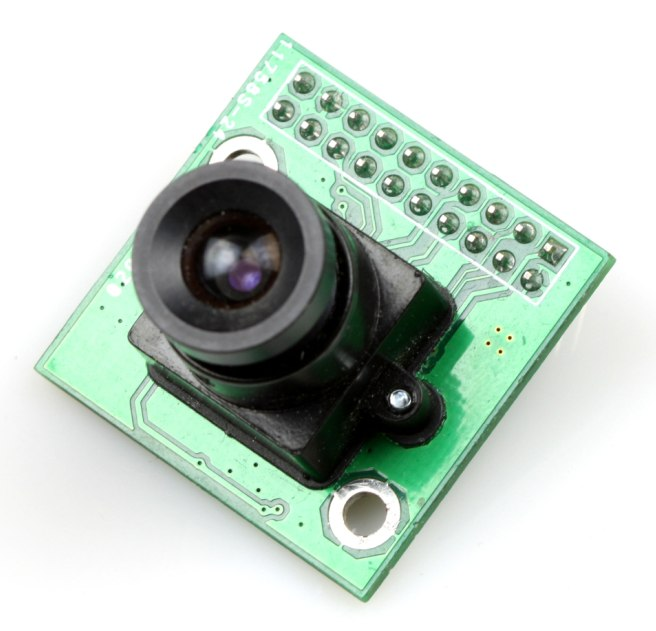
\includegraphics[width=0.5\columnwidth]{figures/mt9d111-m12}
        \caption{Arducam camera module (MT9D111 sensor).}
        \label{fig:mt9d111-module}
    \end{center}
\end{figure}

\begin{figure}[!ht]
    \begin{center}
        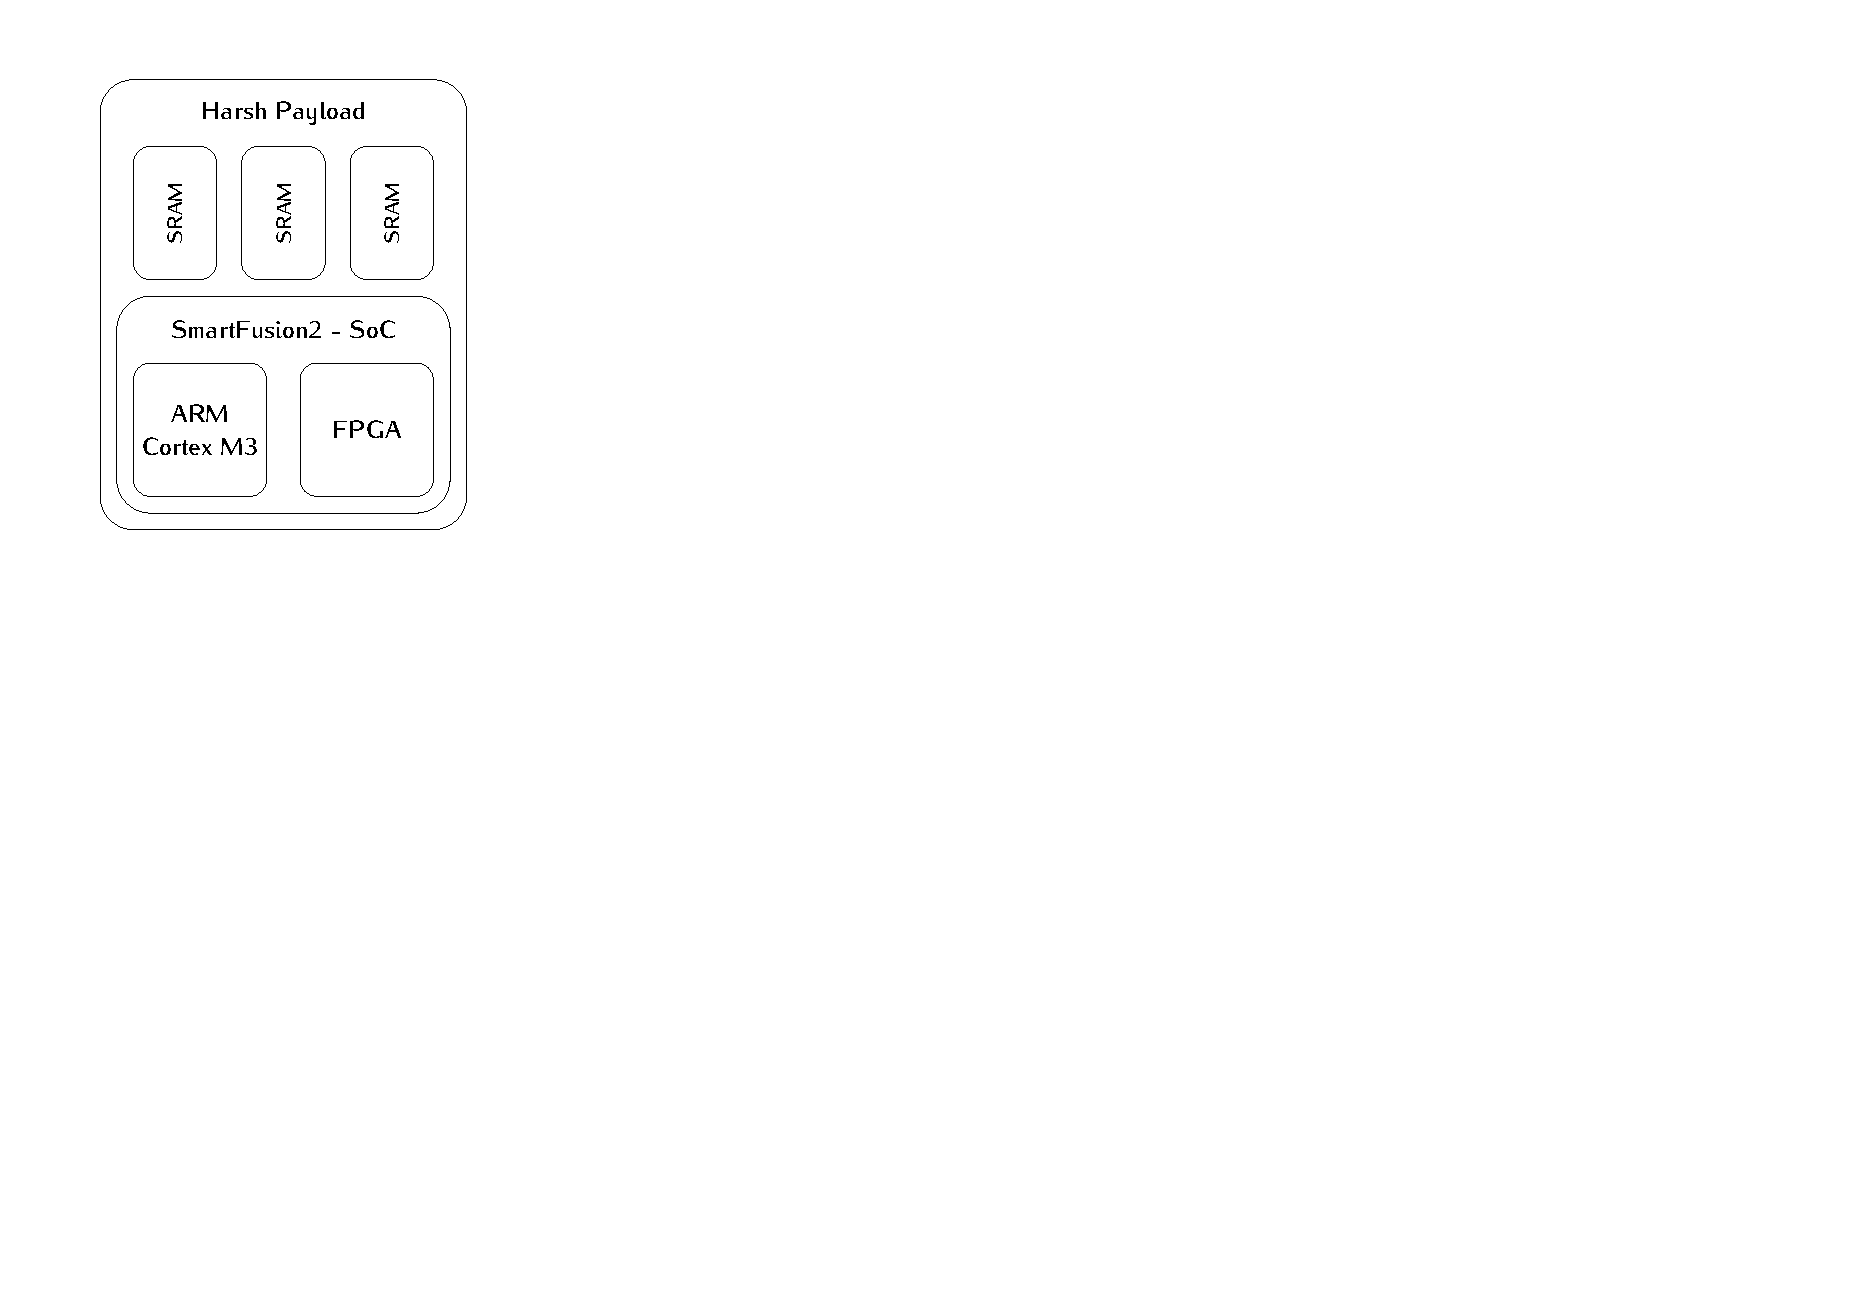
\includegraphics[width=0.5\columnwidth]{figures/harsh-block-diagram}
        \caption{Block diagram of the platform to be used in the proposed experiment.}
        \label{fig:experiment-platform-block-diagram}
    \end{center}
\end{figure}

%In order to accomplish this objectives, the payload is designed to follow the OBDH DaughterBoard standard of SpaceLab, which defines the connectors, shape and size of the board. This standard allows the utilization of the module throughout future SpaceLab core missions in reason of its low space occupation inside the CubeSat, being considered further as an expansion module instead of a payload experiment. A picture of the exploded view of the harsh payload and the OBDH can be seen in \autoref{fig:harsh-payload-integration}.

Also, due to the mission limited power budget, the developed board should consider reduce power consumption and define clever power management strategies. In addition, methods for anti latch-up, a type of short circuit which can occur inside an IC, are considered in the design. Therefore, combining all these requirements, the payload architecture consists of the following modules: a control and management subsystem, operated by a System-On-a-Chip (SoC) solution with an integrated FPGA, power converters for properly voltage level supply, anti latch-up circuitry, communication and interface buses, debug module and the SDRAM memory chips.

\begin{figure}[!htb]
    \begin{center}
        \subfigure[Image example.\label{fig:var-filter-img}]{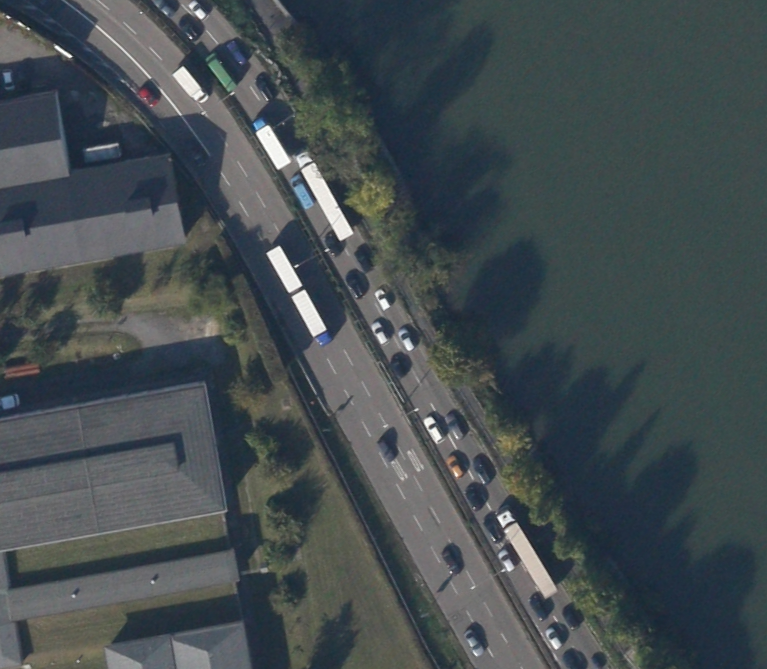
\includegraphics[width=\columnwidth]{figures/MOS15}}

        \subfigure[Variance filter result.\label{fig:var-filter-res}]{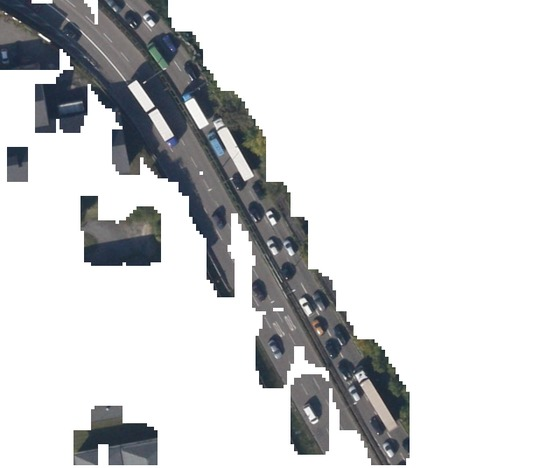
\includegraphics[width=\columnwidth]{figures/var-filter-output}}
        \caption{Variance filter example.}
        \label{fig:variance-filter-example}
    \end{center}
\end{figure}

\begin{figure*}[!ht]
    \begin{center}
        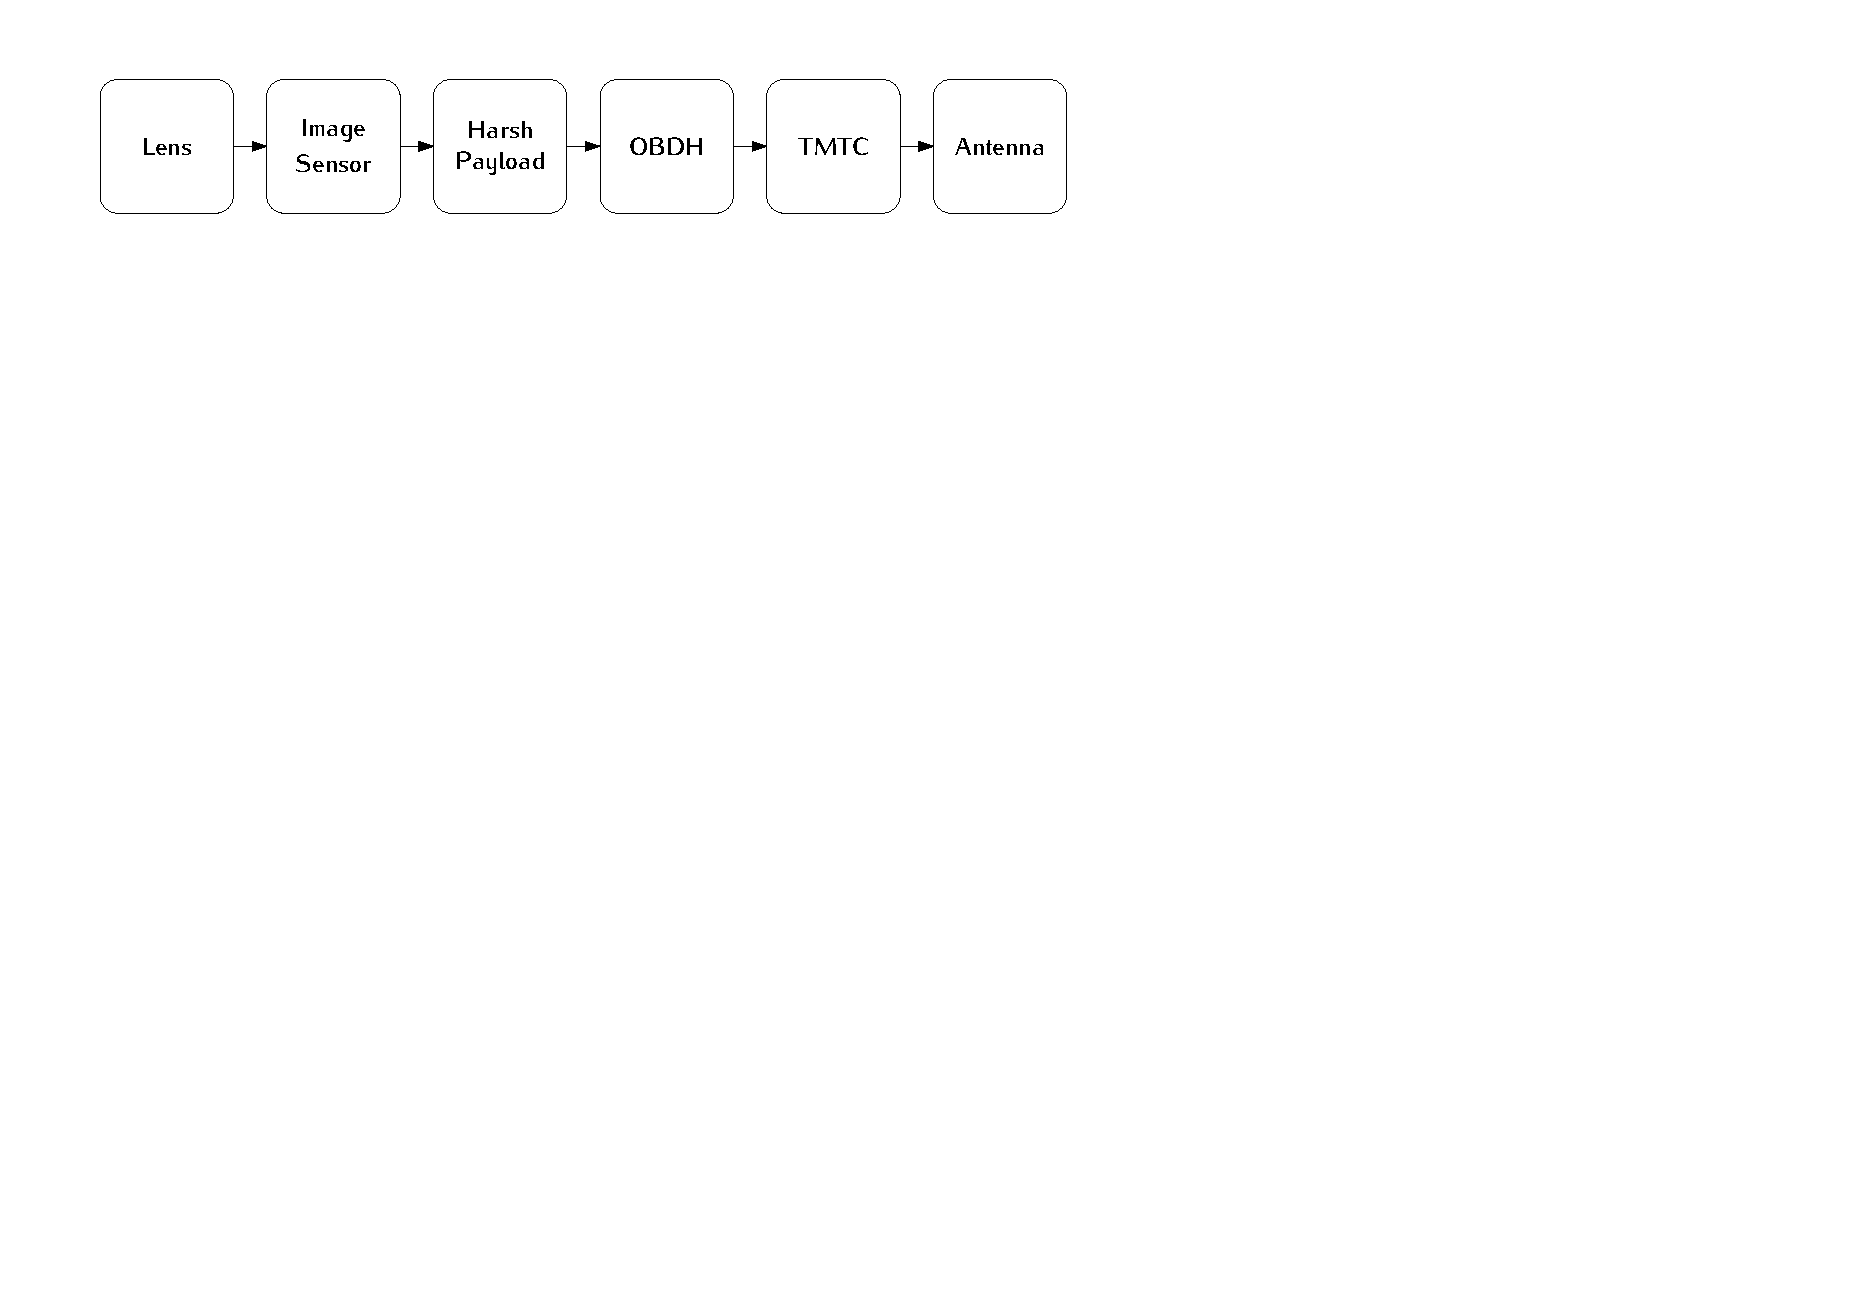
\includegraphics[width=0.8\textwidth]{figures/experiment-block-diagram}
        \caption{Block diagram of the experiment's hardware.}
        \label{fig:experiment-block-diagram}
    \end{center}
\end{figure*}

